% section Extension of the framework to density level set estimation
%
% PLEASE DON'T TOUCH THE ACRONYMS (EVERY \ac, \acp, \acs, etc.) THEY WORK FINE!
% IF YOU DON'T SEE THEM COMPILE WITH
%
% scons --kind=draft
%
% AND YOU SHOULD SEE THEM
%
% IF IT DOESNT COMPILE ON YOUR COMPUTER GET OVER IT AND DO NOT TOUCH THEM! THEY
% ARE EXPANDED AT THE RIGHT MOMENT, WITH THE PLURAL FORM IF NEEDED ON COMPUTERS
% WHERE IT COMPILES.
%
% NOTE: IF YOU DONT WANT TO USE THE COMMAND \ac, \acp, \acs, ... \ IT'S FINE.
% JUST DONT TOUCH THE EXISTING ONE.
%
%
% bias is put in section 3
% -------------------------------
%Adding a bias helps to recover proper quantiles (left figure).
%Here a linear kernel $k_{\inputspace}$. For the hyperparameter kernel
%$k_{\hyperparameter}$ a Gaussian kernel with a large $\sigma$ has been chosen,
%such that all quantile have the same shape. To separate the quantile levels and
%avoid the pathological case on the right figure, a bias term must be added.
%
% In this section we demonstrate the efficiency of the proposed approach on 3
% tasks, Quantile Regression, Level-Set estimation and Cost-Sensitive learning.
%
%
In this section we provide numerical examples illustrating the efficiency of
the proposed \acs{ITL} approach.\footnote{The code is available at
    \url{https://bitbucket.org/RomainBrault/itl}.} We used the following
datasets in our experiments: \par
\begin{figure*}[!tp]
    \centering
    \centering\resizebox{!}{.5\linewidth}{%
        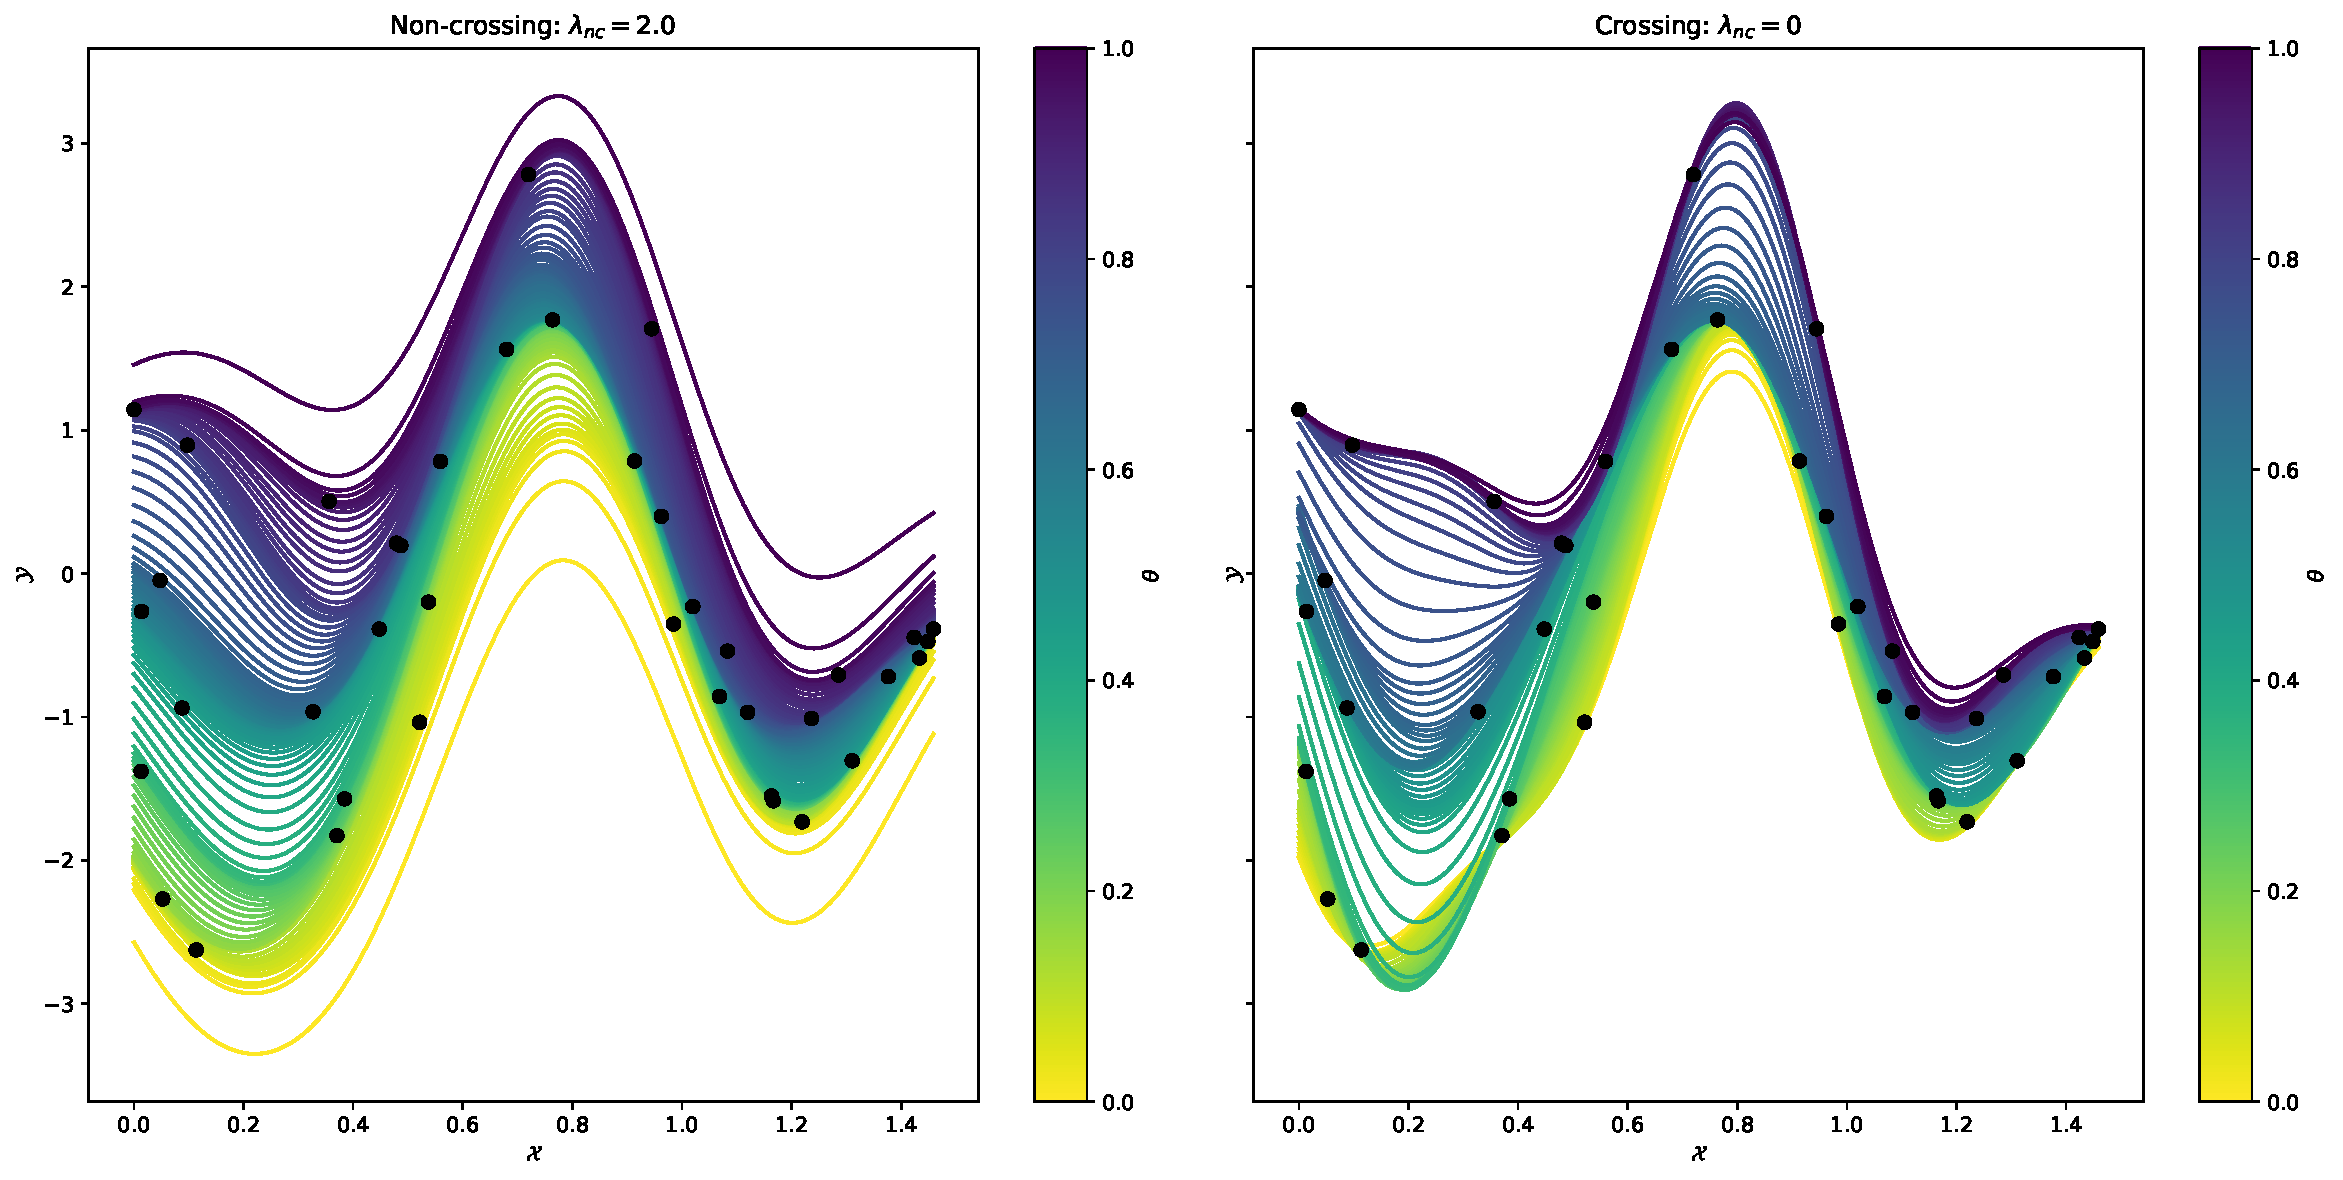
\includegraphics{src/fig/autogen/iqr_crossing.pdf}}
    \caption{Impact of crossing penalty on toy data. Left plot: strong
    non-crossing penalty ($\lambda_{\text{nc}}=10$). Right plot: no
    non-crossing penalty ($\lambda_{\text{nc}}=0)$. The plots show $100$
    quantiles of the continuum learned, linearly spaced between $0$ (blue) and
    $1$ (red). Notice that the non-crossing penalty does not provide crossings
    to occur in the regions where there is no points to enforce the penalty
    (\acs{eg} $x\in\closedinterval{0.13}{0.35}$). This phenomenon is
    alleviated by the regularity of the model.  \label{figure:iqr_crossing}}
\end{figure*}
%
% \subsection{Datasets}
% %
% Concerning the disavantages of \acs{L-BFGS-B}, the convergence rate is still
% not well understood and there is no proof of convergence is the non-smooth
% case, although it performs empirically well. To adapt to our case we propose to
% smooth using the infimal convolution $\square$ of the loss with the smooth
% function $\abs{\cdot}^2$, $\kappa\in\reals_+$. Then we define the Huberized
% absolute $\psi_1$ value as
% \begin{align}\label{equation:huber_absolute_value}
%     \psi_{1}^\kappa(p) \defeq \left(\kappa \abs{\cdot} \square \frac{1}{2}
%     \abs{\cdot}^2 \right)(p)
%     \hiderel{=}
%     \begin{cases}
%         \frac{1}{2\kappa}p^2 & \text{if $\abs{p} \le \kappa$} \\
%         \abs{p} - \frac{\kappa}{2} & \text{otherwise.}
%     \end{cases}
% \end{align}
% And the Huberized positive part $\psi_+$ as
% \begin{align}\label{equation:huber_positive_part}
%     \psi_{+}^\kappa(p) \defeq \left(\kappa\abs{\cdot}_+ \square\frac{1}{2}
%     \abs{\cdot}^2 \right)(p)
%     \hiderel{=}
%     \begin{cases}
%         \frac{1}{2\kappa}\abs{p}_+^2 & \text{if $p \le \kappa$} \\
%         p - \frac{\kappa}{2} & \text{otherwise.}
%     \end{cases}
% \end{align}
% Notice that this \say{trick} guarantees theoreticaly the L-BFGS-B and doesn't
% impact much the theoretical properties of the estimator for small values of
% $\kappa$ as shown in the supplementary material \cref{figure:kappa_study}.
% \begin{remark}
%     minimizing the Huberized pinball loss
%     \begin{align*}
%         \parametrizedcost{\hyperparameter}(y, h(x))=\abs{\hyperparameter -
%         \indicator{\reals_{-}}(y - h(x))}\psi_1^\kappa(y - h(x)),
%     \end{align*}
%     yields the quantiles when $\kappa=0$ and the expectiles when
%     $\kappa\to+\infty$. The intermediates values are known as M-quantiles
%     \citep{breckling1988m}.
% \end{remark}
% In practice we noticed that this smoothing trick is unnecessary and the
% \acs{L-BFGS-B} convergences well on non-smooth objective as long as the
% iterates are never evaluated on non-differentiable points (see
% \cref{remark:initialization}).  Moreover non-smooth L-BFGS-B exists
% \citep{skajaa2010limited,keskar2017limited} and propose an implementation based
% on the work of \citet{keskar2017limited}.  Due to the lack of efficient
% implementation this algorithm, while adapted to handle non-smooth problem, is
% slower than the stantard \acs{L-BFGS-B}.
% \begin{remark}\label{remark:initialization}
%     Concerning the initinalization of the \acs{L-BFGS-B}, we advise to
%     initialize the coefficient randomly. Indeed notice that in the case of
%     Quantile Regression or Level Set estimation $0$ is \emph{exactly} a
%     non-differentiable point leading the optimizer to immediate failure.
% \end{remark}
% %
%
%
\label{paragraph:datasets}
%
%
\begin{itemize}[labelindent=0cm,leftmargin=*,topsep=0cm,partopsep=0cm,
                parsep=2mm,itemsep=0cm]
    \item \acl{QR}: we used
        \begin{inparaenum}[(i)]
            \item a sine synthetic benchmark \citep{sangnier2016joint}: a sine
            curve at $1Hz$ modulated by a sine envelope at $1/3Hz$ and mean
            $1$, distorted with a Gaussian noise of mean 0 and a linearly
            decreasing standard deviation from $1.2$ at $x=0$ to $0.2$ at
            $x=1.5$.
            \item $20$ standard regression datasets from \acs{UCI}.
            %  regression datasets, and three
            % additional ones (quantred, alr3 and MASS) provided by the R
            % software environment.
            %, used to benchmark Joint Quantile Regression
            %\citep{sangnier2016joint}.
            The number of samples varied between $38$ (CobarOre) and $1375$
            (Height).  The observations were standardised to have unit
            variance and zero mean for each attribute.
            %\item[(iii)] the reg-1d regression benchmark of liquidSVM
            %\citep{steinwart2017liquidsvm} with $2000$ samples and $1$
            %attribute.
        \end{inparaenum}
    % \item \acl{CSC}: The Iris \acs{UCI} dataset with $4$ attributes and $150$
    % samples. The two synthetic \textsc{scikit-learn}
    % \citep{pedregosa2011scikit} datasets \textsc{Two-Moons} (noise=$0.4$) and
    % $\textsc{Circles}$ (noise=$0.1$) with both $2$ attributes and $1000$
    % samples. A third synthetic \textsc{scikit-learn} dataset \textsc{Toy}
    % (class sep=$0.5$) with $20$ features ($4$ redundant and $10$ informative)
    % and $n=1000$ samples.
    \item \acl{DLSE}: The Wilt database from the \acs{UCI} repository with
    $4839$ samples and $5$ attributes, and the Spambase \acs{UCI} dataset with
    $4601$ samples and $57$ attributes served as benchmarks.
\end{itemize}
Additional experiments related to the \ac{CSC} problem are provided in \cref{subsection:csc_expe}.
%
\paragraph{Note on Optimization:}
There are several ways to solve the non-smooth optimization problems  associated
to the \ac{QR}, \ac{DLSE} and \ac{CSC} tasks. One could proceed for example by
duality---as it was done in JQR \citet{sangnier2016joint}---, or apply
sub-gradient descent techniques (which often converge quite slowly). In order
to allow unified treatment and efficient solution
% optimise the objective many options are possible. A efficient way of proceeding
% is to rewrite \cref{equations:representer} as a constrained problem and solve
% it in the dual. The main advantage of the dual formulation being that a
% strongly convex non-smooth functional in the primal becomes smooth in the dual,
% leveraging fast convergence algorithms. This is the approach taken by
% \citet{sangnier2016joint}.
% %in using
% %primal-dual algorithms \citep{shalev2013stochastic,sangnier2016joint}.  Another
% %solution is to stay in the primal and apply a Proximal gradient algorithm.
% %
% However this approach lacks of flexibility since for each problem (in the
% proposed framework) a dual formulation must be derived. Moreover although dual
% methods would adapted when $h$ lives in a \ac{RKHS}, it would make little sense
% to use such methods if $h$ is a neural network or a random feature
% \citet{Rahimi2007,brault2016random} (\ac{ie} the kernel trick is inefficient),
% that we plan to study in a near future.
%
% In this context, more flexible approaches solving the problem in the primal
% include sub-gradient descent which only requires to compute the (sub)gradient
% of the objective. Yet this methods are known to have poor convergence rate,
% have no implementable stopping criteria, and requires to finely tune the step
% size. \par
in our experiments we used the \acs{L-BFGS-B} \citep{zhu1997algorithm}
optimization scheme which is widely popular in large-scale learning, with
non-smooth extensions \citep{skajaa2010limited,keskar2017limited}. The
technique requires only evaluation of objective function along with its
gradient, which can be computed automatically using reverse mode automatic
differentiation (as in \citet{abadi2016tensorflow}). To benefit from  from the
available fast smooth implementations \citep{jones2014scipy,fei2014parallel},
we applied an infimal convolution
% $\square$ with $\frac{1}{2}\abs{\cdot}^2$ on
(\seet{subsection:infimal_convo} of the supplementary material) on the
non-differentiable terms of the objective. Under the assumtion that
$m=\mathcal{O}(\sqrt{n})$ (see \cref{proposition:generalization_supervised}),
the complexity per \ac{L-BFGS-B} iteration is $\mathcal{O}(n^2\sqrt{n})$.
An experiment showing the impact of increasing $m$ on a synthetic dataset is
provided in \cref{figure:iqr_m}.
% For the sake of reproducibility we will provide a link to an online repository
% with a Python library written for the experiments.
% The Python library replicating our experiments is available in the supplement.
\par
%
% Notice that evaluating the model $h$ on a batch of point $(x_i)_{i=1}^n$ and
% $(\theta_j)_{j=1}^m$ can be done efficiently using the Kroencker trick:
% \begin{dmath*}
%     (h(x_i)(\theta_j))_{i,j=1}^{n,m} = \mathbf{K}_{\inputspace}
%     \boldsymbol{\alpha} \mathbf{K}_{\hyperparameterspace},
% \end{dmath*}
% where $\mathbf{K}_{\inputspace}$ and $\mathbf{K}_{\hyperparameterspace}$ are
% the Gram matrices of $k_{\inputspace}$ and $k_{\hyperparameterspace}$
% respectively and $\boldsymbol{\alpha}$ is the $n\times m$ matrix of parameters.
% Hence prediction on a batch of inputs of $n$ data and $m$ hyperparameters cost
% $\mathcal{O}(n^2m + m^2n)$ (1), while predicting them independently would cost
%$\mathcal{O}(n^2m^2)$ (2).
% Note that non batch
% optimization methods such as \ac{SGD} pay the price of independent predictions
% (2).
% For quantile regression, $19$ datasets issued from the \acs{UCI} repository and
% 3 R packages are used (quantred, alr3 and MASS). This dataset have been
% proposed to benchmark the Joint Quantile Regression algorithm proposed by
% \citet{sangnier2016joint}. The number of samples of each datasets is relatively
% small: beetween $38$ (CobarOre) and $506$ (BostonHousing). These datasets have
% been standardised to unit variance and zero mean for each attributes. We also
% used the synthetic data proposed in \citet{sangnier2016joint}'s work: a sine
% curve at $1Hz$ modulated by a sine envelope at $1/3Hz$ and mean $1$, distorted
% with a Gaussian noise of mean 0 and a linearly decreasing standard deviation
% from $1.2$ at $x=0$ to $0.2$ at $x=1.5$. Eventually we considered the dataset
% reg-1d of liquidSVM \refmissing with $2000$ samples and $1$ attribute.\par For
% classification we illustrated Cost-Sensitive learning on the classical Iris
% dataset considering only the features petal length and petal width. Finally we
% used the \acs{UCI} dataset Wilt with $4839$ samples and $5$ attributes to
% benchmark the our proposed algorithm for level-set estimation.
% %
%
%
% \paragraph{\acl{QR}:}
% This section is about our experiments in quantile regression.
% \ifthenelse{\isundefined{\typepdf}}{
%     \begin{center}
%         \begin{figure*}[t]
%           \centering
%           \resizebox{!}{0.5\linewidth}{%
%               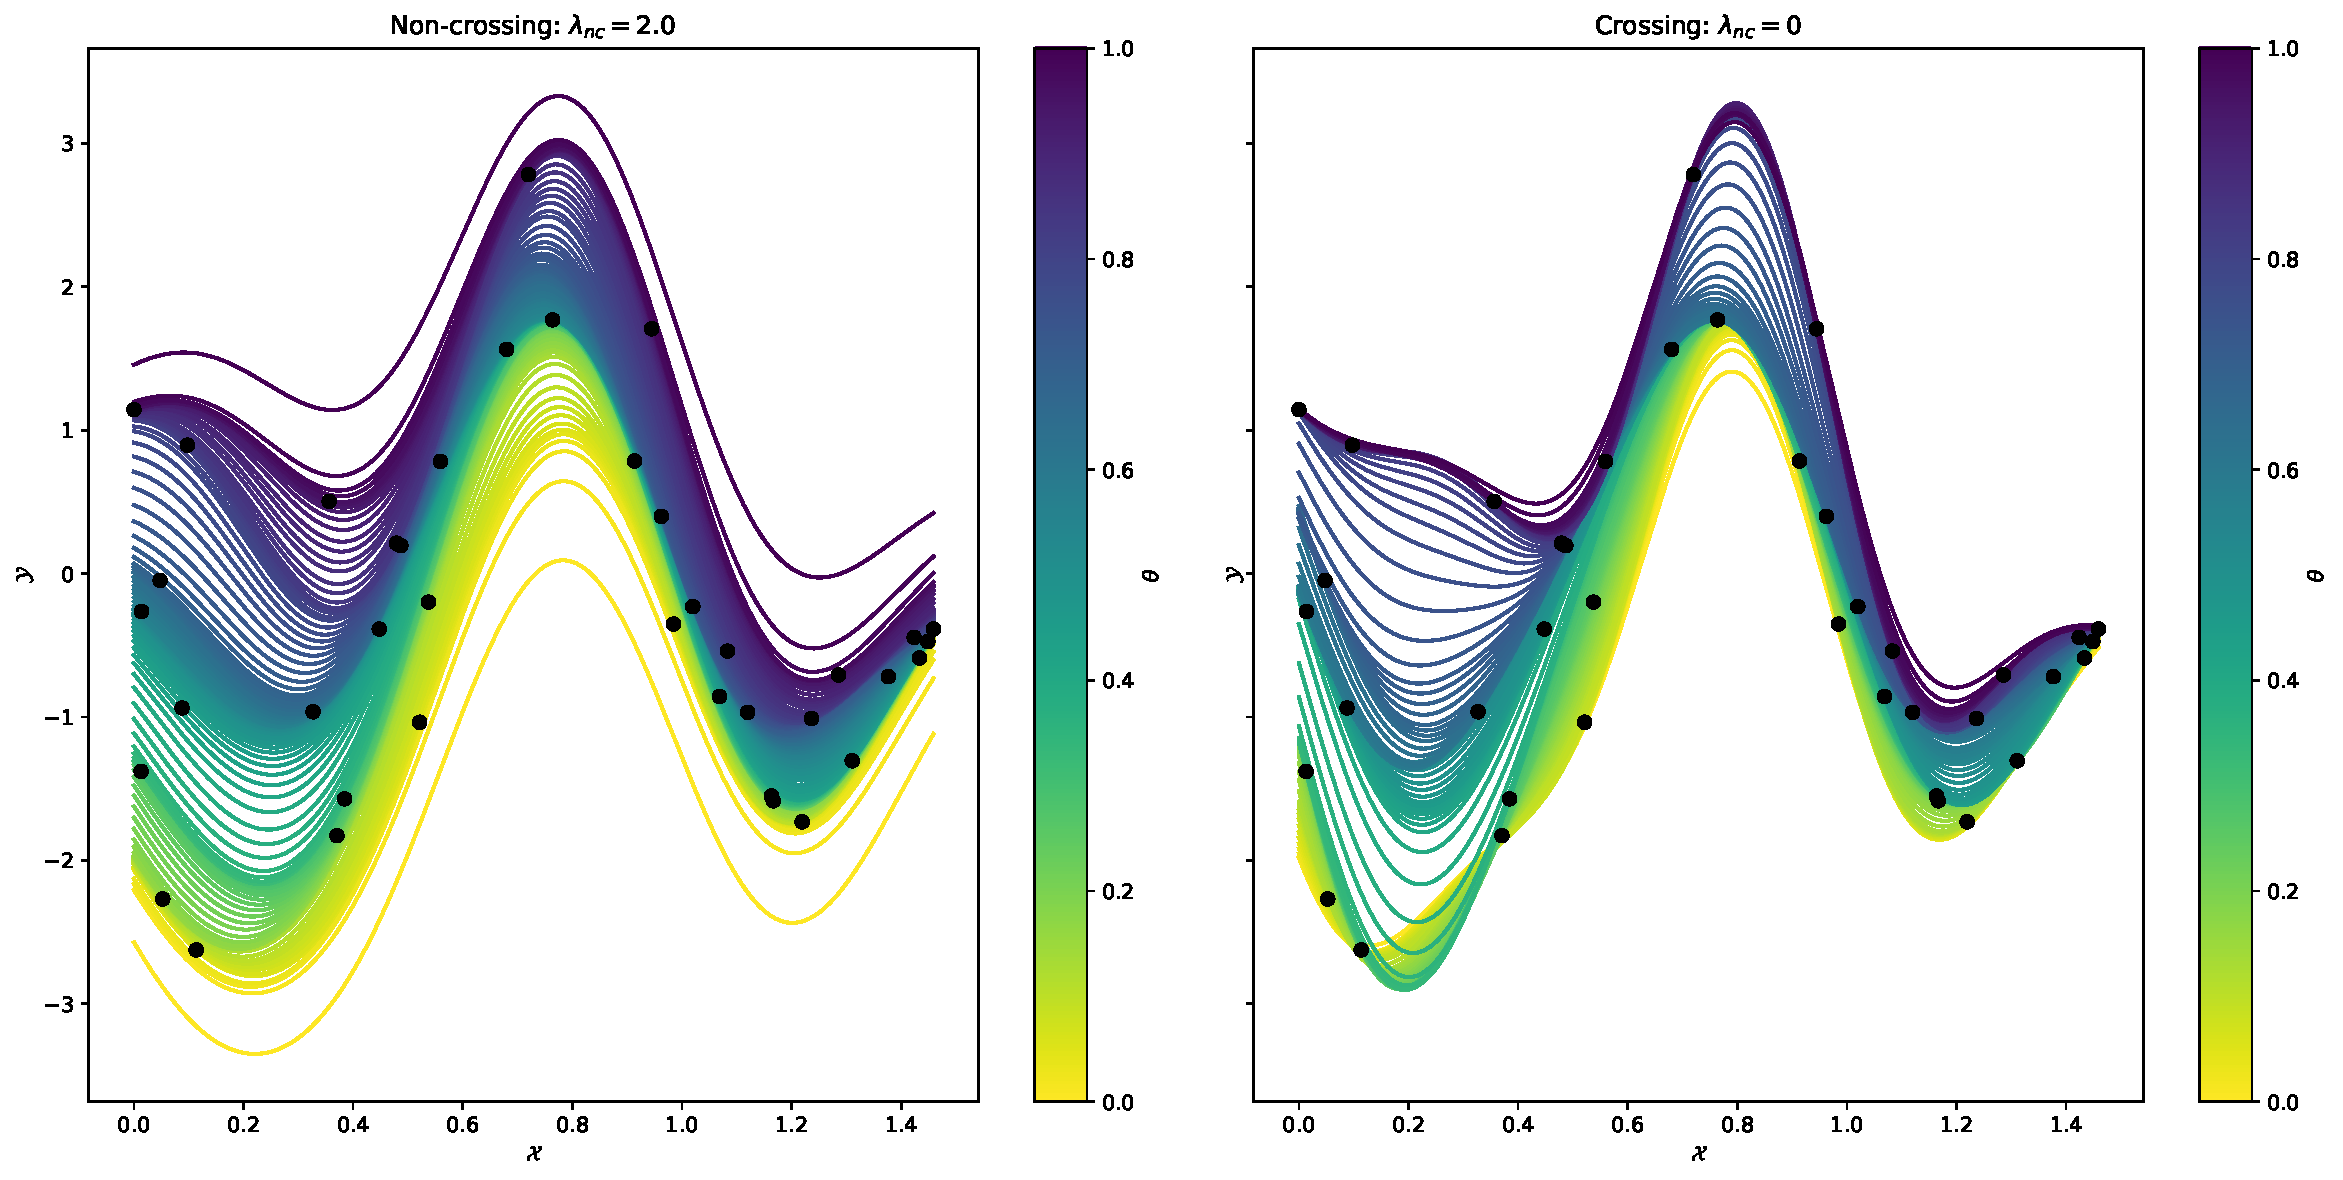
\includegraphics{src/fig/autogen/iqr_crossing.eps}}
%               \caption{Impact of crossing penalty on toy data. Left plot: strong
%               non-crossing penalty ($\lambda_{\text{nc}}=2$). Right plot: no
%               non-crossing penalty ($\lambda_{\text{nc}}=0)$. The plots show $100$
%               quantiles of the continuum learned, linearly spaced
%               between $0$ (blue) and $1$ (red).
%               \label{figure:iqr_crossing}}
%         \end{figure*}
%     \end{center}
%             }{
%         \begin{center}
%             \begin{figure*}[t]
%               \centering
%               \resizebox{!}{0.5\linewidth}{%
%                   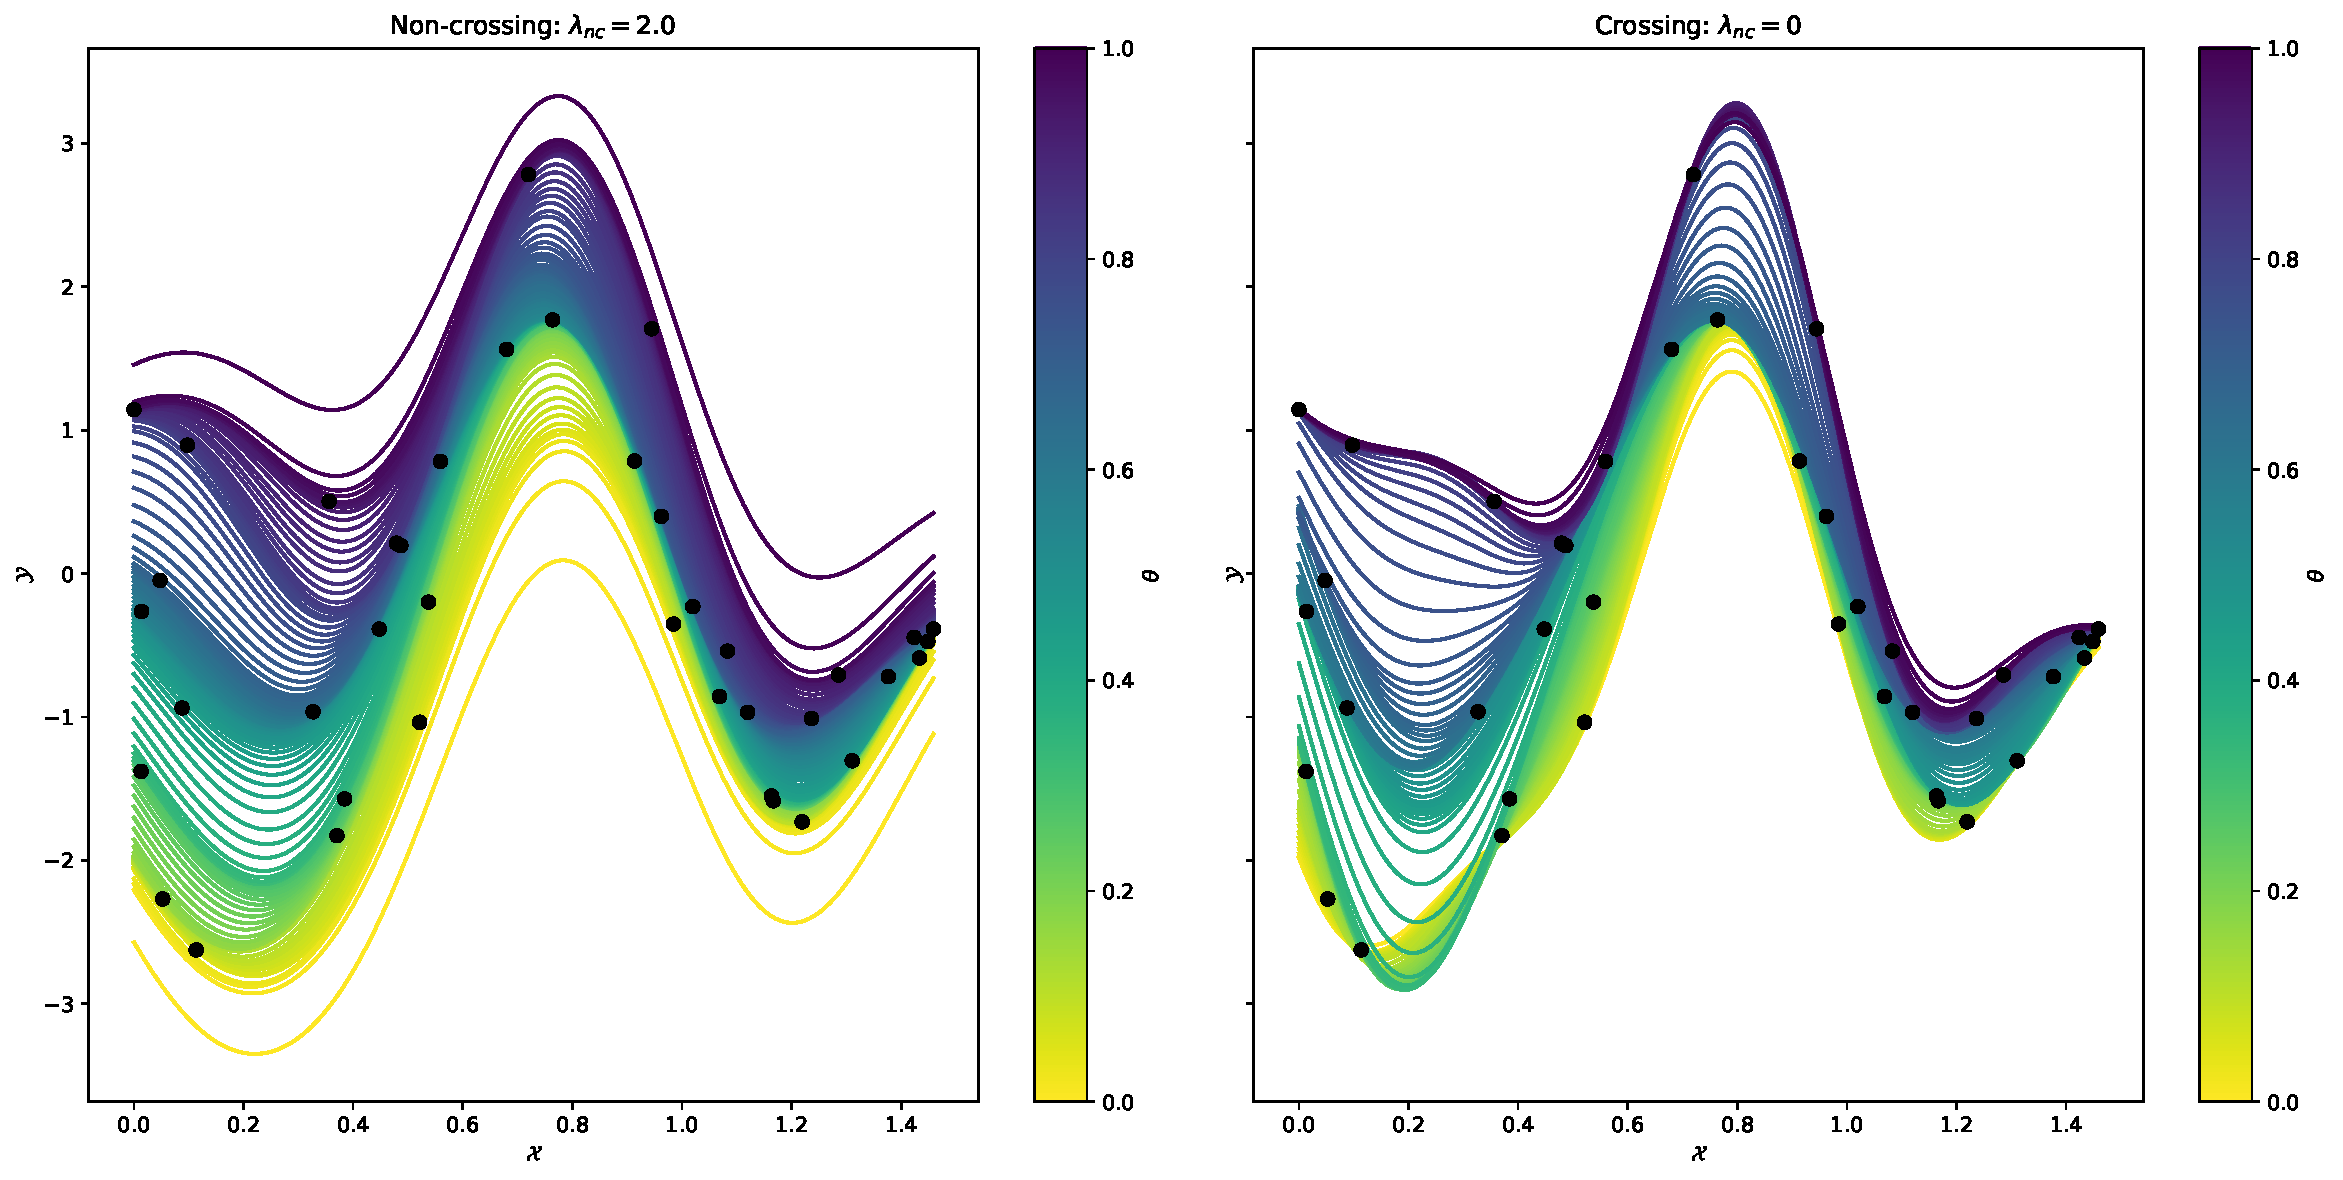
\includegraphics{src/fig/autogen/iqr_crossing.pdf}}
%                   \caption{Impact of crossing penalty on toy data. Left plot: strong
%                   non-crossing penalty ($\lambda_{\text{nc}}=2$). Right plot: no
%                   non-crossing penalty ($\lambda_{\text{nc}}=0)$. The plots show $100$
%                   quantiles of the continuum learned, linearly spaced
%                   between $0$ (blue) and $1$ (red).
%                   \label{figure:iqr_crossing}}
%             \end{figure*}
%         \end{center}
% }
% Our proposed framework contains the objective minimized by
% \citet{sangnier2016joint} when $\mu$ is chosen to be a discrete probability
% measure. Below we investigate the efficiency of learning with a continuum of
% hyperparameters, and also compare it with that of the cited work: see Remark-2
% in \cref{section}.
\paragraph{\ac{QR}:}
% While a quantile function by
% definition is monotonically increasing, the estimate based on finite samples
% might violate this property as it was observed
% \citep{takeuchi2006nonparametric}. Existing solutions mitigating this
% bottleneck include the application of non-crossing inducing constraints, as
% expressed for example by the
% crossing loss $\hcost_{\text{nc}}(h, (\hyperparameter_j)_{j=1}^m) \defeq
% \sum_{j=1}^{m-1}\frac{1}{n}\sum_{i=1}^n \abs{h_{x_i}(\theta_{j + 1}) -
% h_{x_i}(\theta_{j})}_+$, where $\hyperparameter_1 < \ldots < \hyperparameter_m$
% and $h_x(\theta)\defeq h(x)(\theta)$. Intuitively, non-crossing  is enforced by
% constraining the quantile level $h(x_i)(\hyperparameter_{j+1})$ to be smaller
% than the quantile level $h(x_i)(\theta_j)$ for $\hyperparameter_{j+1} >
% \hyperparameter_j$ and for all $x_i$ in the training set. In our case, when a
% continuum of quantiles are being learned, we propose to penalize the risk when
% the derivative of $h$ \acs{wrt} $\hyperparameter$ is negative, as encoded by
% the
% \begin{align}\label{equation:non_crossing}
%     \Omega_{\text{nc}}(h) \defeq
%     \lambda_{nc}\int_{\inputspace}\int_{\hyperparameterspace}\abs{
%     -\frac{\partial h}{\partial \hyperparameter}
%     (x)(\theta)}_+d\mu(\hyperparameter)d\probability(x)
% \end{align}
% penalty. When $\probability\defeq\probability_{X}$~; \cref{equation:non_crossing}
% can be approximated using the same anchors and weights than the one obtained to
% integrate the loss function
% %\begin{align}\label{equation:non_crossing_sampled}
% $\widetilde{\Omega}_{\text{nc}}(h) =
% \frac{\lambda_{nc}}{n}\sum_{i=1}^n\sum_{j=1}^mw_j\abs{ -\frac{\partial
% h}{\partial \hyperparameter} (x_i)(\theta_j)}_+$.
%\end{align}
% Notice that with this penalty, the representer theorem still applies since by
% linearity of the sum this term can be incorporated into the loss.
 % The final loss function is given in \cref{table:integrated_risks}.
The efficiency of the non-crossing penalty is illustrated in
\cref{figure:iqr_crossing} on the synthetic sine wave dataset described in
\cref{paragraph:datasets} where $n=40$ and $m=20$ points have been generated.
Many crossings are visible on the right plot, while they are almost not
noticible on the left plot, using the non-crossing penalty.
% The model was trained with a
% bias.  For $k_{\inputspace}$ a Gaussian kernel was used,
% $k_{\hyperparameterspace}$ and $k_{b}$ were Laplacian kernels. All bandwidths
% were set to $10$ to emphasise the possible crossings.
%
% \paragraph{\ac{QR}-Real Data Experiments:}
% \begin{table*}[!htbp]
%     \caption{\acs{ICSC} vs Independent (IND)-\acs{CSC}. Higher is
%     better.\label{table:csc_results}}
%     \addtolength{\tabcolsep}{-3pt}
%     \renewcommand{\arraystretch}{0.8}% Tighter
%     \begin{center}
%         \begin{tiny}
%             \begin{sc}
%                 \resizebox{.7\textwidth}{!}{%
%                 \begin{tabular}{cccccccc}
%                     \toprule
%                     \multirow{2}{*}{Dataset} & \multirow{2}{*}{Method} &
%                     \multicolumn{2}{c}{$\theta=-0.9$} &
%                     \multicolumn{2}{c}{$\theta=0$} &
%                     \multicolumn{2}{c}{$\theta=+0.9$} \\
%                     \cmidrule(lr){3-4} \cmidrule(lr){5-6} \cmidrule(lr){7-8} &
%                     & \textsc{sensitivity} & \textsc{specificity} &
%                     \textsc{sensitivity} & \textsc{specificity} &
%                     \textsc{sensitivity} & \textsc{specificity} \\
%                     \midrule
%                     \multirow{ 2}{*}{\textsc{Two-Moons}} & IND &
%                     $0.3\pm0.05$ & $0.99\pm0.01$ & $0.83\pm0.03$ &
%                     $0.86\pm0.03$ & $0.99\pm0$ & $0.32\pm0.06$ \\
%                                                 & \acs{ICSC} & $0.32\pm0.05$ &
%                     $0.99\pm0.01$ & $0.84\pm0.03$ & $0.87\pm0.03$ & $1\pm0$ &
%                     $0.36\pm0.04$  \\
%                     \multirow{ 2}{*}{\textsc{Circles}} & IND & $0\pm0$
%                     & $1\pm0$ & $0.82\pm0.02$ & $0.84\pm0.03$ & $1\pm0$ &
%                     $0\pm0$ \\
%                                               & \acs{ICSC} & $0.15\pm0.05$ &
%                     $1\pm0$ & $0.82\pm0.02$ & $0.84\pm0.03$ & $1\pm0$ &
%                     $0.12\pm0.05$  \\
%                     \multirow{ 2}{*}{\textsc{Iris}} & IND &
%                     $0.88\pm0.08$ & $ 0.94\pm0.06$ & $0.94\pm0.05$ &
%                     $0.92\pm0.06$ & $0.97\pm0.05$ & $0.87\pm0.06$\\
%                                            & \acs{ICSC} & $0.89\pm0.08$ &
%                     $0.94\pm0.05$ & $0.94\pm0.06$ & $0.92\pm0.05$ &
%                     $0.97\pm0.04$ & $0.90\pm0.05$
%                     \\
%                     \multirow{ 2}{*}{\textsc{Toy}} & IND &
%                     $0.51\pm0.06$ & $ 0.98\pm0.01$ & $0.83\pm0.03$ &
%                     $0.86\pm0.03$ & $0.97\pm0.01$ & $0.49\pm0.07$\\
%                                            & \acs{ICSC} & $0.63\pm0.04$ &
%                     $0.96\pm0.01$ & $0.83\pm0.03$ & $0.85\pm0.03$ &
%                     $0.95\pm0.02$ & $0.61\pm0.04$
%                     \\
%                     \bottomrule
%                 \end{tabular}}
%             \end{sc}
%         \end{tiny}
%     \end{center}
%     \addtolength{\tabcolsep}{3pt}
%     \renewcommand{\arraystretch}{1.0}% Tighter
% \end{table*}
%Iris
%0.8858054348091039 0.0806029709975442 0.9400301823413251 0.04812224196301379
%0.9372082019207957 0.06341081656928274 0.9168173004941926 0.05335694923606509
%0.9746338458032612 0.04107852166305085 0.9009818889847182 0.04807169907101462
%
%0.8823921963260792 0.0787696895824724 0.9478441114476902 0.055036149869177174
%0.9410937811369595 0.05642030750892981 0.920800249007726 0.05751560544731357
%0.9714963403135816 0.0455514664670911 0.8783034656145408 0.06411936345519713
%
%Synthetic
%0.6278744008652377 0.03660640971083982 0.9605477305391755 0.014915860047845663
%0.829262713786789 0.0294835926729205 0.8541487435432024 0.028283429496290875
%0.9483602058321796 0.016302585748520965 0.613858182907852 0.04241654101931668
%
%0.5139200084602886 0.061290011465502725 0.9779168024658391 0.011980934760118698
%0.8298119969812278 0.031137552936250906 0.8570540311177968 0.02724535972357056
%0.9720299291680792 0.014123740663262562 0.4921282191346739 0.06719490115704468V
Concerning our real-world examples, to study the efficiency of the proposed
scheme in quantile regression the
following experimental protocol was applied. Each dataset
(\cref{paragraph:datasets}) was splitted randomly into a training set (70\%)
and a test set (30\%). We optimized the hyperparameters by minimizing a
$5$-folds cross validation with a Bayesian optimizer\footnote{We used a
Gaussian Process model and minimized the Expected improvement. The optimizer
was initialized using $27$ samples from a Sobol sequence and ran for $50$
iterations.} (For further details \seet{subsection:proto_exp}).
Once the hyperparameters were obtained, a new regressor was
learned on the whole training set using the optimized hyperparameters. We
report the value of the pinball loss and the crossing loss on the test set for
three methods: our technique is called $\infty$-\ac{QR}, we refer to
\citet{sangnier2016joint}'s approach as  \ac{JQR}, and independent learning
(abbreviated as IND-\ac{QR}) represents a further baseline. \par
%
% For $\infty$-\ac{QR}, $k_{\inputspace}$, $k_{\hyperparameterspace}$ were Gaussian
% kernels. We set a bias term $k_b=k_{\hyperparameterspace}$. The hyperparameters
% optimized were $\lambda$, the weight of the ridge penalty,
% $\sigma_\inputspace$, the input kernel parameter, and
% $\sigma_\hyperparameterspace$, the output kernel parameter. They were optimized
% in the (log)space of $\closedinterval{10^{-6}}{10^{6}}^3$. The non-crossing
% constraint $\lambda_{nc}$ was set to $1$. The model was trained on the
% continuum $\Theta=\openinterval{0}{1}$ using QMC and Sobol sequences. \par
% %
% For \ac{JQR] we similarly chose two Gaussian kernels. The optimized hyperparameters
% were the same as for $\infty$-\ac{QR}.
% % are also the bandwidth of the Gaussian kernel acting on the inputs, the bandwith
% % of the kernel acting on the outputs, and the regularization tradeoff $\lambda$
% % which where optimized in the (log)space $\closedinterval{10^{-6}}{10^{6}}^3$.
% The quantiles learned were $\theta\in\Set{0.1, 0.3, 0.5, 0.7, 0.9}$.\par
% %
% For the INDEPENDENT baseline, we trained independently a non-paramatric
% quantile estimator as described in \citet{takeuchi2006nonparametric}. A
% Gaussian kernel was used and its bandwidth was optimized in the (log)space of
% $\closedinterval{10^{-6}}{10^6}$. No non-crossing was enforced. \par
%
We repeated $20$ simulations (different random training-test splits); the
results are also compared using a Mann-Whitney-Wilcoxon test. A summary is
provided in \cref{table:quantile_results}.
%
%Thanks to the optimization of the hyperparameters the comparison of the methods
%is more fair and
%
% ******* massaged until this point: Zoltan *******
% \zs{I do not see what is happening below. The pinball loss should be small on the test set (smaller is better). But e.g., for the stated improvements, CRABS: 11 (JQR) << 14 ($\infty$-QR), CPUS: 7 (JQR) << 13 ($\infty$-QR), ???}
% \rb{We improved on 4 datasets over Sangnier for *all* methods $\infty$-QR JQR and
% INDEP. This suggest that our experimental protocol is more robust. In our
% experimental setting statitisticaly significant differences between methods not
% visible for the pinball score EXCEPT for crabs and cpus where we perform worst.
% In terms of crossing loss we do significantly better than JQR on two datasets. }
% Overall we improved on the results reported on
% \citet{sangnier2016joint} (especially on the datasets cpus, crabs, engel and
% mcycle). Moreover the difference between the methods in terms of value of the
% pinball loss is less significant. We notice that learning a continuum rather
% than specific quantiles is only significantly behind the state of the art on
% two of the nineteen proposed datasets (\acs{pval}
% $<.25\%$)\footnote{Because the experiments were conducted on $19\approx20$
% datasets, false discovery are more likely to happen. To take this phenomenon
% into account we used the Bonferroni correction and divided the classical
% \acs{pval} of $5\%$ by $20$.}. This suggest that one must be carefull and
% investigate the data and not replace blindly learning for specific
% hyperparameters by their continuum counterpart. Also note that the evaluation
% criteria does not play in our favour, while other method focused their training
% precisely on the tested quantile, ours had to account for the whole
% continuum.\par
% %
% On the other hand when looking at the crossing penalty, learning on a continuum
% and imposing non-crossing outperformed the baseline on eleven datasets
% (\acs{pval} $<.25\%$) and JQR on two datasets. This suggest that
% learning on a continuum allows to enforce stronger structure properties on the
% model learned.
%
Notice that while \ac{JQR} is tailored to predict finite many quantiles, our
$\infty$-\ac{QR} method estimates the \emph{whole quantile function} hence
solves a more challenging task.  Despite the more difficult problem solved, as
\cref{table:quantile_results} suggest that the performance in terms of pinball
loss of $\infty$-\ac{QR} is comparable to that of the state-of-the-art JQR on
all the twenty studied benchmarks, except for the `crabs' and `cpus' datasets
(\acs{pval} $<0.25\%$). In addition, when considering the non-crossing penalty
one can observe that $\infty$-\ac{QR} outperforms the IND-\ac{QR} baseline on
eleven datasets (\acs{pval} $<0.25\%$) and \ac{JQR} on two datasets. This
illustrates the efficiency of the constraint based on the continuum scheme.
%
\paragraph{\ac{DLSE}:}
To assess the quality of the estimated model by $\infty$-\acs{OCSVM}, we
illustrate the $\theta$-property \citep{scholkopf2000new}: the proportion of
inliers has to be approximately $1-\hyperparameter$ ($\forall \hyperparameter
\in (0,1)$).  For the studied datasets (Wilt, Spambase) we used the raw inputs
without applying any preprocessing.  Our input kernel was the exponentiated
$\chi^2$ kernel $k_{\inputspace}(x, z)\defeq \exp\left(-\gamma_{\inputspace}
\sum_{k=1}^d(x_k - z_k)^2/(x_k + z_k)\right)$ with bandwidth
$\gamma_{\inputspace}=0.25$.  A Gauss-Legendre quadrature rule provided the
integral approximation in \cref{equation:integrated_cost}, with $m=100$
samples. We chose the Gaussian kernel for $k_{\hyperparameterspace}$; its
bandwidth parameter $\gamma_{\hyperparameterspace}$ was the $0.2-$quantile of
the pairwise Euclidean distances between the $\theta_j$'s obtained via the
quadrature rule.  The margin (bias) kernel was $k_b=k_{\hyperparameterspace}$.
As it can be seen in Fig.~\ref{fig:iocsvm_nu_novelty}, the $\theta$-property
holds for the estimate which illustrates the efficiency of the proposed
continuum approach for density level-set estimation.
\begin{figure}[htbp]
    \centering
    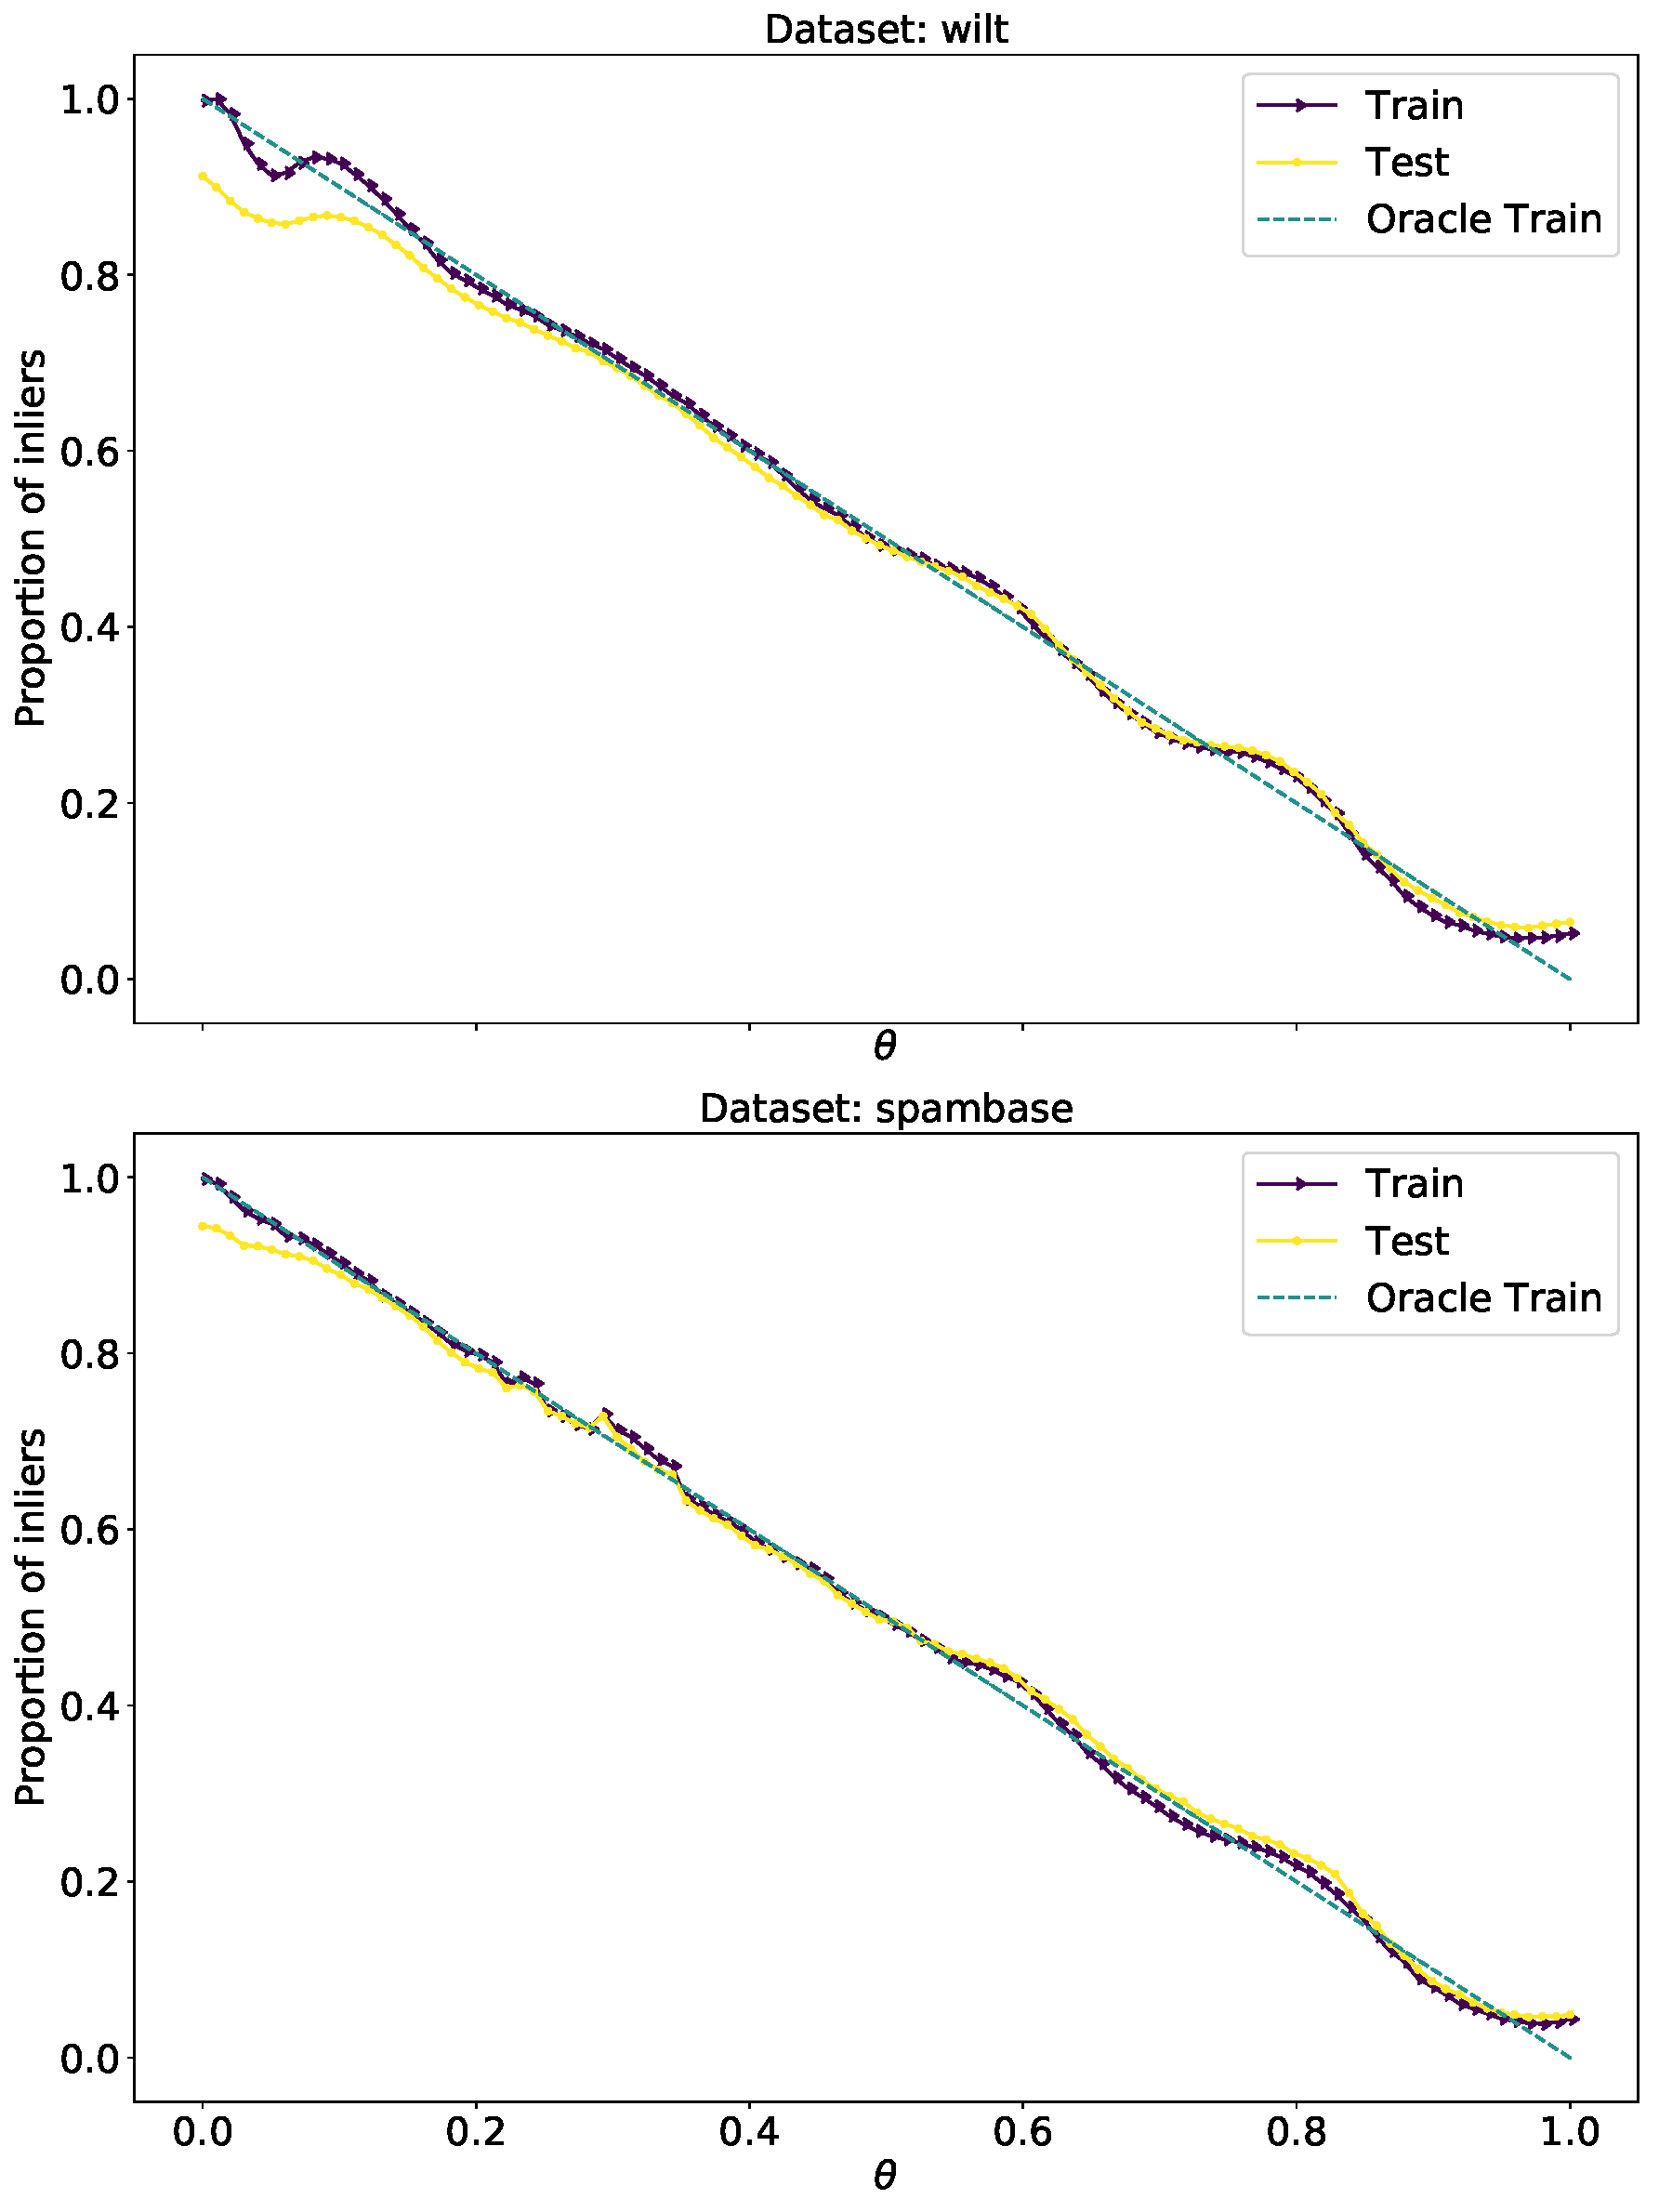
\includegraphics[width=\textwidth]{src/fig/autogen/iocsvm_nu.pdf}
    \caption{\acl{DLSE}: the $\theta$-property is
    approximately satisfied. \label{fig:iocsvm_nu_novelty}}
\end{figure}
%
%  This two
% experiments suggest that the \acs{L-BFGS-B} can cope well with non-smooth
% objective and on rather large and high dimensional datasets. Second the
% $\theta$-property seems to be recovered suggesting that the proposed integrated
% cost is a valid generalization to learn on the continuum of $\theta\in(0, 1)$.
%
% \paragraph{\acl{CSC}:}
% %
% % NOTE on takeuchi parametric. we fall in his framework
% %
% % IF:
% %               * The loss is convex but piecewise linear, does not depend on
% %               theta AND the weights depends on theta but are piecewise linear
% %               (eg CSC)
% %               * The loss is convex depends on theta but is piecewise linear
% %               and the weights depends on theta and are piecewise constant eg.
% %               quantile
% %
% %
% As detailed in \cref{section:infinite_tasks}, \acl{CSC} on a continuum
% $\hyperparameterspace = \closedinterval{-1}{1}$ that we call \ac{ICSC}
% can be tackled by our proposed technique.  In this case, the hyperparameter
% $\hyperparameter$ controls the tradeoff between the importance of the correct
% classification with labels $-1$ and $+1$. When $\hyperparameter = -1$,
% class $-1$ is emphasized; the probability of correctly classified instances
% with this label (called specificity) is desired to be $1$.  Similarly, for
% $\hyperparameter = +1$, the probability of correct classification of samples
% with label $+1$ (called sensitivity) is ideally $1$.\par
% %
% To illustrate the advantage of (infinite) joint learning we used two synthetic
% datasets \textsc{Circles} and \textsc{Two-Moons} and the \acs{UCI}
% \textsc{Iris} dataset. We chose $k_{\inputspace}$ to be a Gaussian kernel with
% bandwidth $\sigma_{\inputspace}=(2\gamma_{\inputspace})^{(-1/2)}$ the median of
% the Euclidean pairwise distances of the input points \citep{jaakkola1999using}.
% $k_{\hyperparameterspace}$ is also a Gaussian kernel with bandwidth
% $\gamma_{\hyperparameterspace}=5$.  We used $m=20$ for all datasets.
% %In order to illustrate the advantage of the joint learning we used the petal
% %length and petal width features from the Iris dataset.  We chose
% %$k_{\inputspace}$ to be the Gaussian kernel with bandwidth
% %$\gamma_{\inputspace}=1$ and $k_{\hyperparameter}= k_b$ to be a Laplacian
% %kernel with bandwidth $\gamma_{\hyperparameter}=\gamma_{b}=1$.
% As a baseline we trained independently 3 \acl{CSC} classifiers with
% $\hyperparameter\in\Set{-0.9,0, 0.9}$. We repeated $50$ times a random $50-50\%$
% train-test split of the dataset and report the average test error and standard
% deviation (in terms of sensitivity and specificity) \par
% %
% Our results are illustrated in \cref{table:csc_results}. For $\theta=-0.9$, both
%  independent and joint learners give the desired $100\%$ specificity; the
% joint \acl{CSC} scheme however has significantly higher sensitivity value
% ($15\%$ vs $0\%$) on the dataset \textsc{Circles}. Similar conclusion holds for the
% $\theta=+0.9$ extreme: the ideal sensitivity is reached by both techniques, but
% the joint learning scheme performs better in terms of specificity ($0\%$ vs
% $12\%$) on the dataset \textsc{Circles}.
%In addition, it
%is interesting to observe that higher sensitivity and specificity values are
%obtained for even the $\hyperparameter=0$ value when none of the classes are
%favoured by the hyperparameter. These results show the efficiency of the
%proposed \ac{ICSC} Learning scheme.
%\begin{figure}[tb]
    %\centering
    %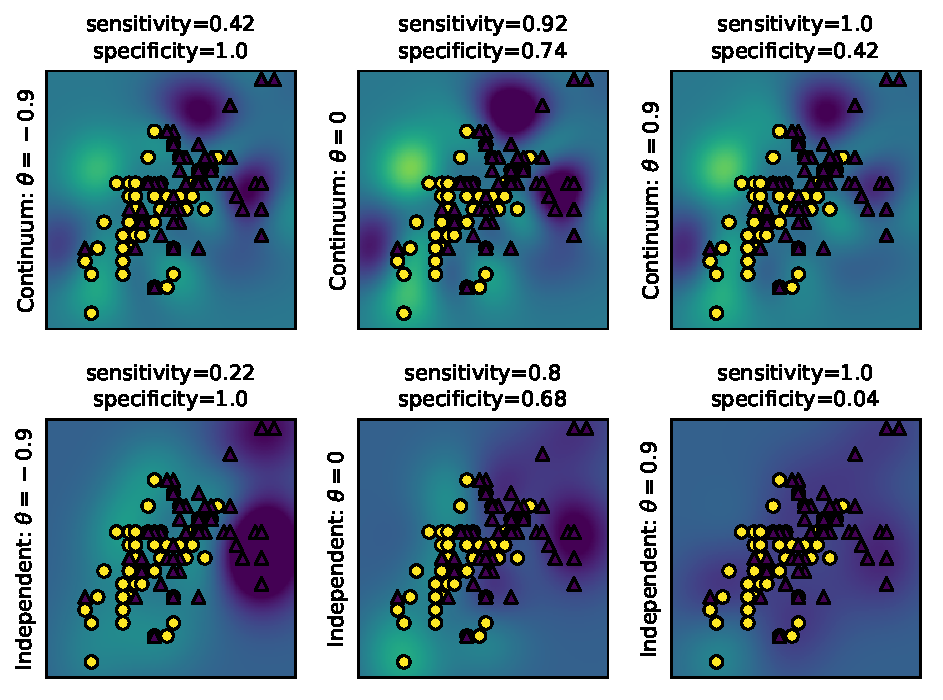
\includegraphics[angle=-90,width=\textwidth]{src/fig/autogen/icsl_vs.pdf}
    %\caption{\ac{CSC}, Iris dataset. Left: independent learning:
    %$\theta\in\Set{-1, 0, 1}$; right: infinite learning.
    %\label{figure:icsl_vs}}
%\end{figure}
%
%
% Cost Sensitive Classification on a continuum, proposed by
% \citet{takeuchi2013parametric} can also be tackled within our framework. Yet
% since we dot not have the restriction of using a piecewise linear loss
% function, it can handle losses such as the smoothed squared hinge losse
% proposed in \cref{table:integrated_risks}. To illustrate this setting we
% proposed an experiment which could have been tackled in Takeuchi's framework
% using the hinge loss (non-smooth).
% We learned independently 3 SVM classifiers
% on the features petal length and petal width of the Iris dataset, for
% $\theta\in\Set{0, .5, 1}$. For our method, we learned on the continuum $(0,
% 1)$, sampling the points from a Sobol sequence. We choosed $k_{\inputspace}$ to
% be a Gaussian kernel with bandwidth $\gamma_{\inputspace}=1$ and
% $k_{\hyperparameter}= k_b$ to be a Laplacian kernel with bandwidth
% $\gamma_{\hyperparameter}=\gamma_{b}=1$.\par
%
% For $\theta=-1$ and $\theta=1$ learning on a continuum allows to recover
% $100\%$ specificity (respectfully $100\%$ sensitivity), while keeping the
% sensitivity (respectfully specificity) significantly higher.  Surprisingly this
% is also true when $\theta=0$ which does not favour sensitivity nor specificity.
